\section{Results}

The fixed effects models without the year effect we ran for this paper all yielded significant coefficients for our high turnover/pace variable (see Table 3). Depending on the number of control variables included, the effect size ranges from 2.14-2.41. None of our included control variables is significant at the 5\% level. Our variabels explain between 18-26\% of the within variance. Revenue accounts for the brunt of the between variance at around 45\%. The Hausman test indicates that a fixed effect model is an appropriate choice for models 2-4, and the F statistic is significant in all but the third model.\footnote{See: \log}

\begin{center}
	
	=================
	
	= Insert Table 3 here =
	
	=================
	
	\begin{table}[] \center
\caption{} 
\label{} 
\begin{tabular}{llllll}
& Model 1 & Model 2 & Model 3 & Model 4 & Model 5 \\
\hline
High Turnover / Pace		& 2.41^*  & 2.17^*  & 2.07^*  & 2.14^*  & 1.91      \\
Revenue       				&         & 0       & 0       & 0       & 0         \\
CEO Exit      				&         &         & 0.75    & -0.7    & 0.66      \\
CEO Exit during				&         &         & 0.75    & -1.32   &           \\
CEO Exit one year before	&         &         & 0.75    & 1.19    &           \\
Year						&         &         &         &         &  0.53     \\
F statistic   				& 7^*     & 3.48^*  &  2.84   & 5.20^*^*& 3.08^*    \\
R-sq within   				& 0.18    & 0.22    &  0.23   & 0.26    &  0.25     \\
R-sq between  				& 0.01    & 0.45    &  0.46   & 0.49    & 0.44      \\
R-sq Overall       			& 0.00    & 0.43    &  0.44   & 0.47    & 0.23      \\
\end{tabular}
\end{table}

	
	
\end{center}

The effect size captures the increase in recalls to be expected from one more year of high turnover/pace in the years preceding the observation period leads to around two additional recalls in that period. For instance, if company A has one year of high turnover/pace in the period of 2007-2010 and 12 recalls take place between 2011-2013, then if the number of high pace years between 2011-2013 was 2, we would expect the number of recalls to grow to 14 in the years 2014-2017. However, since the effect size decreases and becomes insignificant when the year effect is included,  at least some of the findings in model 2-4 might be explainable by autocorrelation.

As we have a low number of obserations, we were interested in the leverage of individual data points. Figures 1-3 show the effect of change in the independent variable on change in the depended variable. As evident from the graphs, two outliers account for the majority of the effect. When these outliers are removed, the relationship between the independent and dependent variable disappears.

\begin{center}
	=================
	
	= Insert Figure 1 here =
	
	=================
	
	=================
	
	= Insert Figure 2 here =
	
	=================
	
	=================
	
	= Insert Figure 3 here =

	=================
\end{center}

\begin{figure}
	\caption{}
	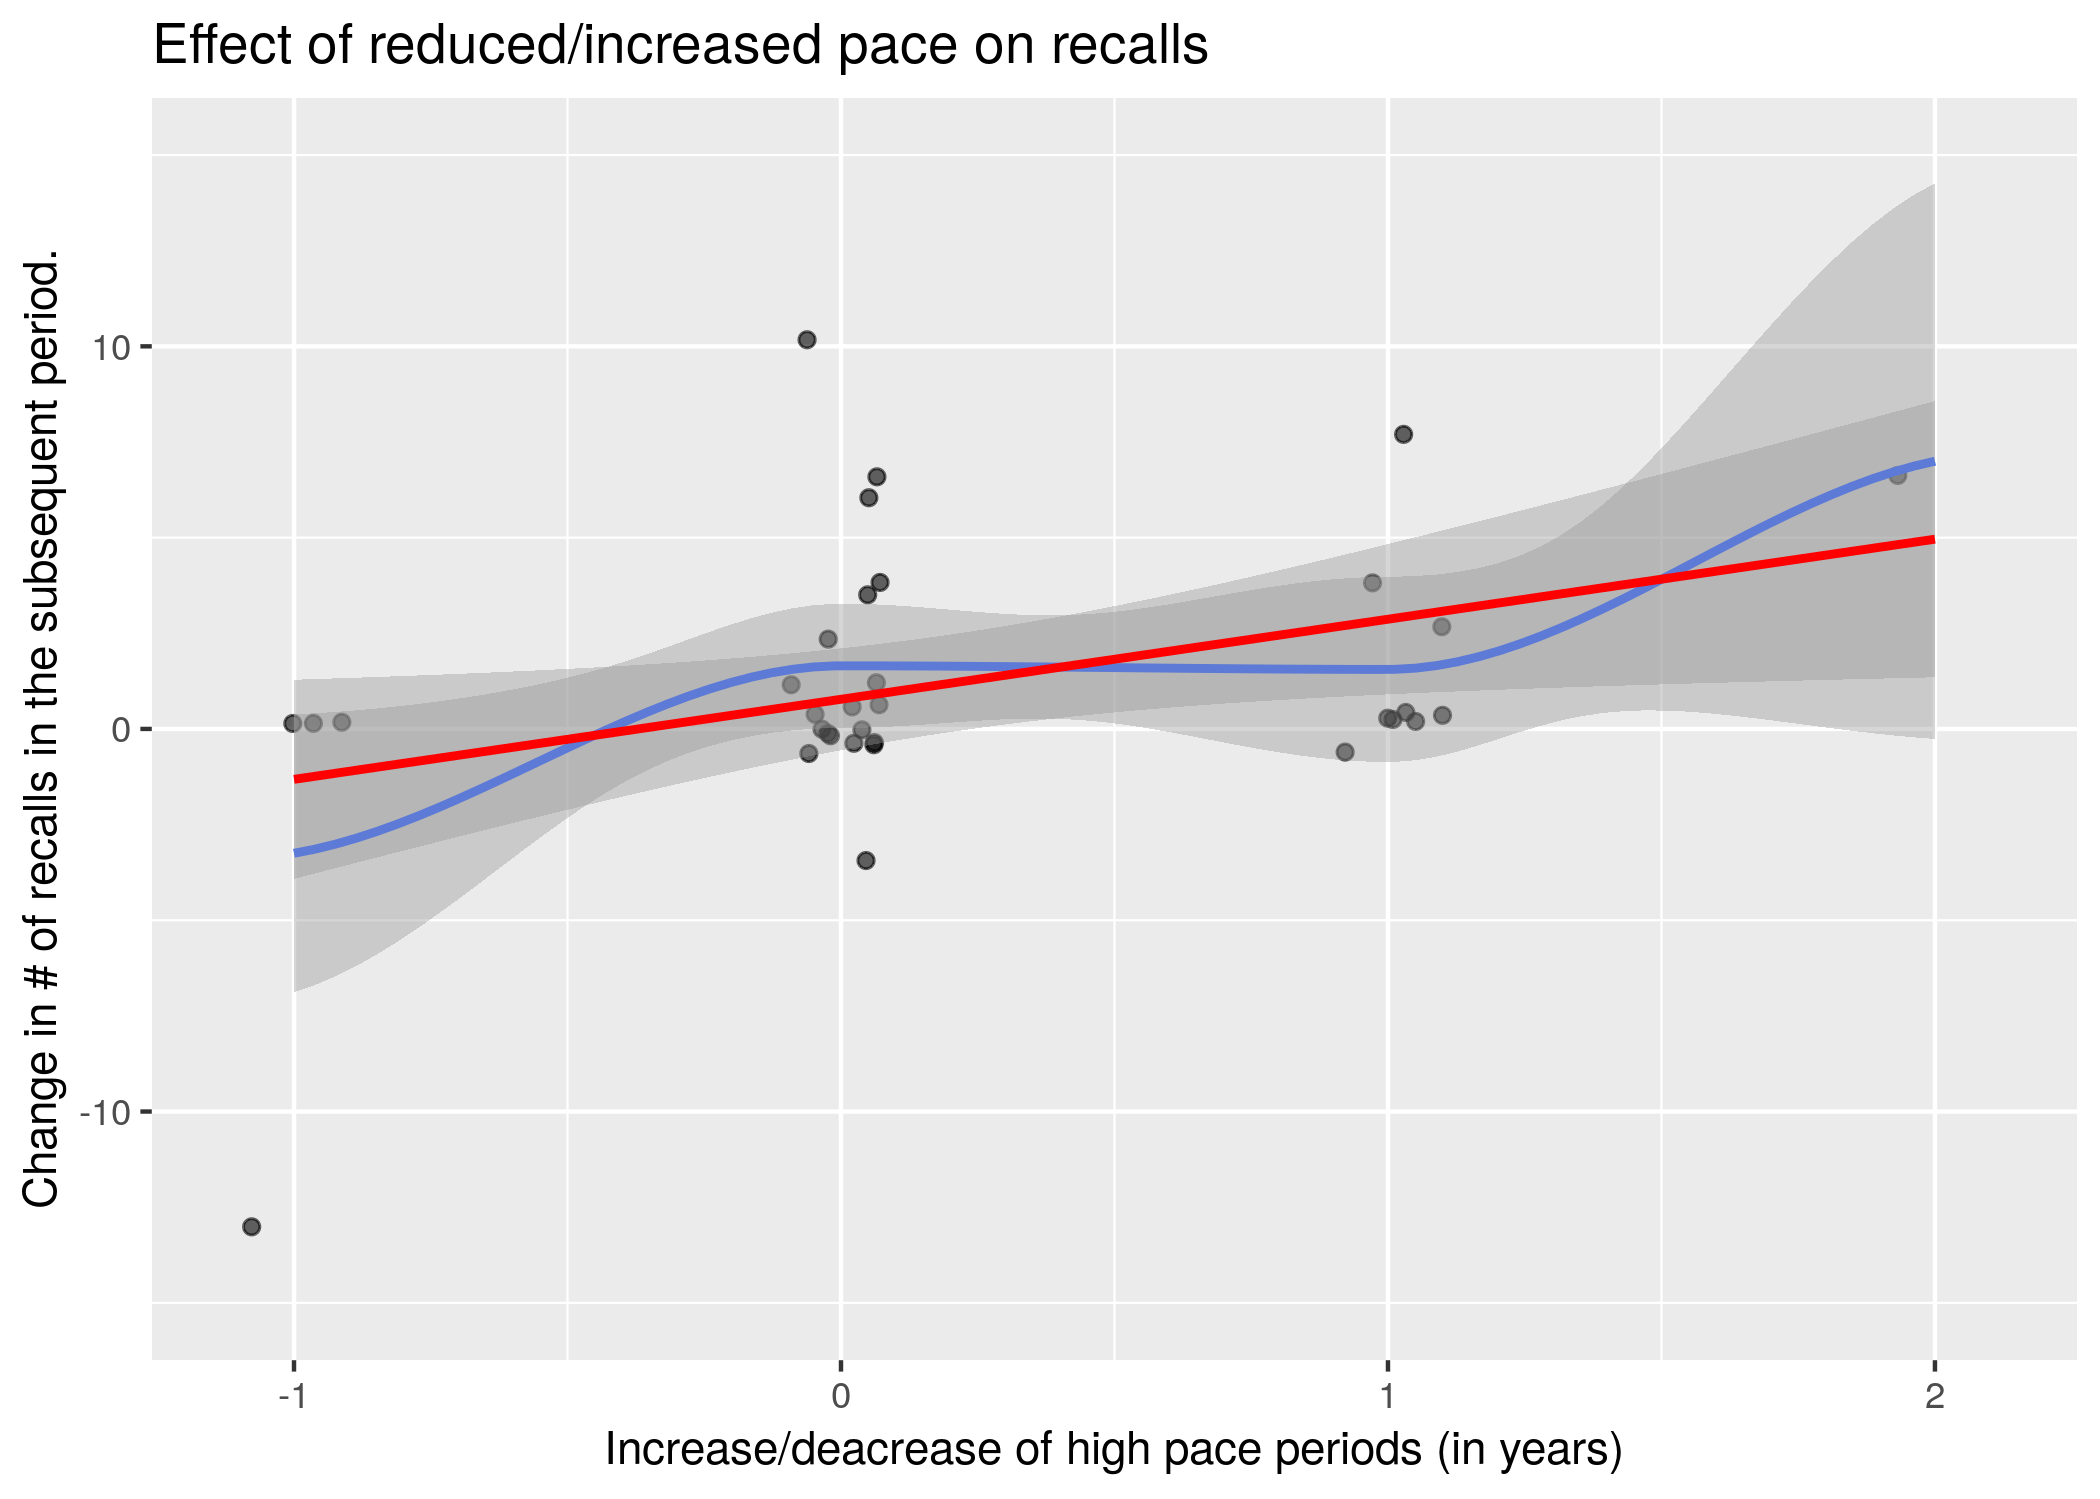
\includegraphics{illustrations/graph1.png}
\end{figure}

\begin{figure}
	\caption{}
	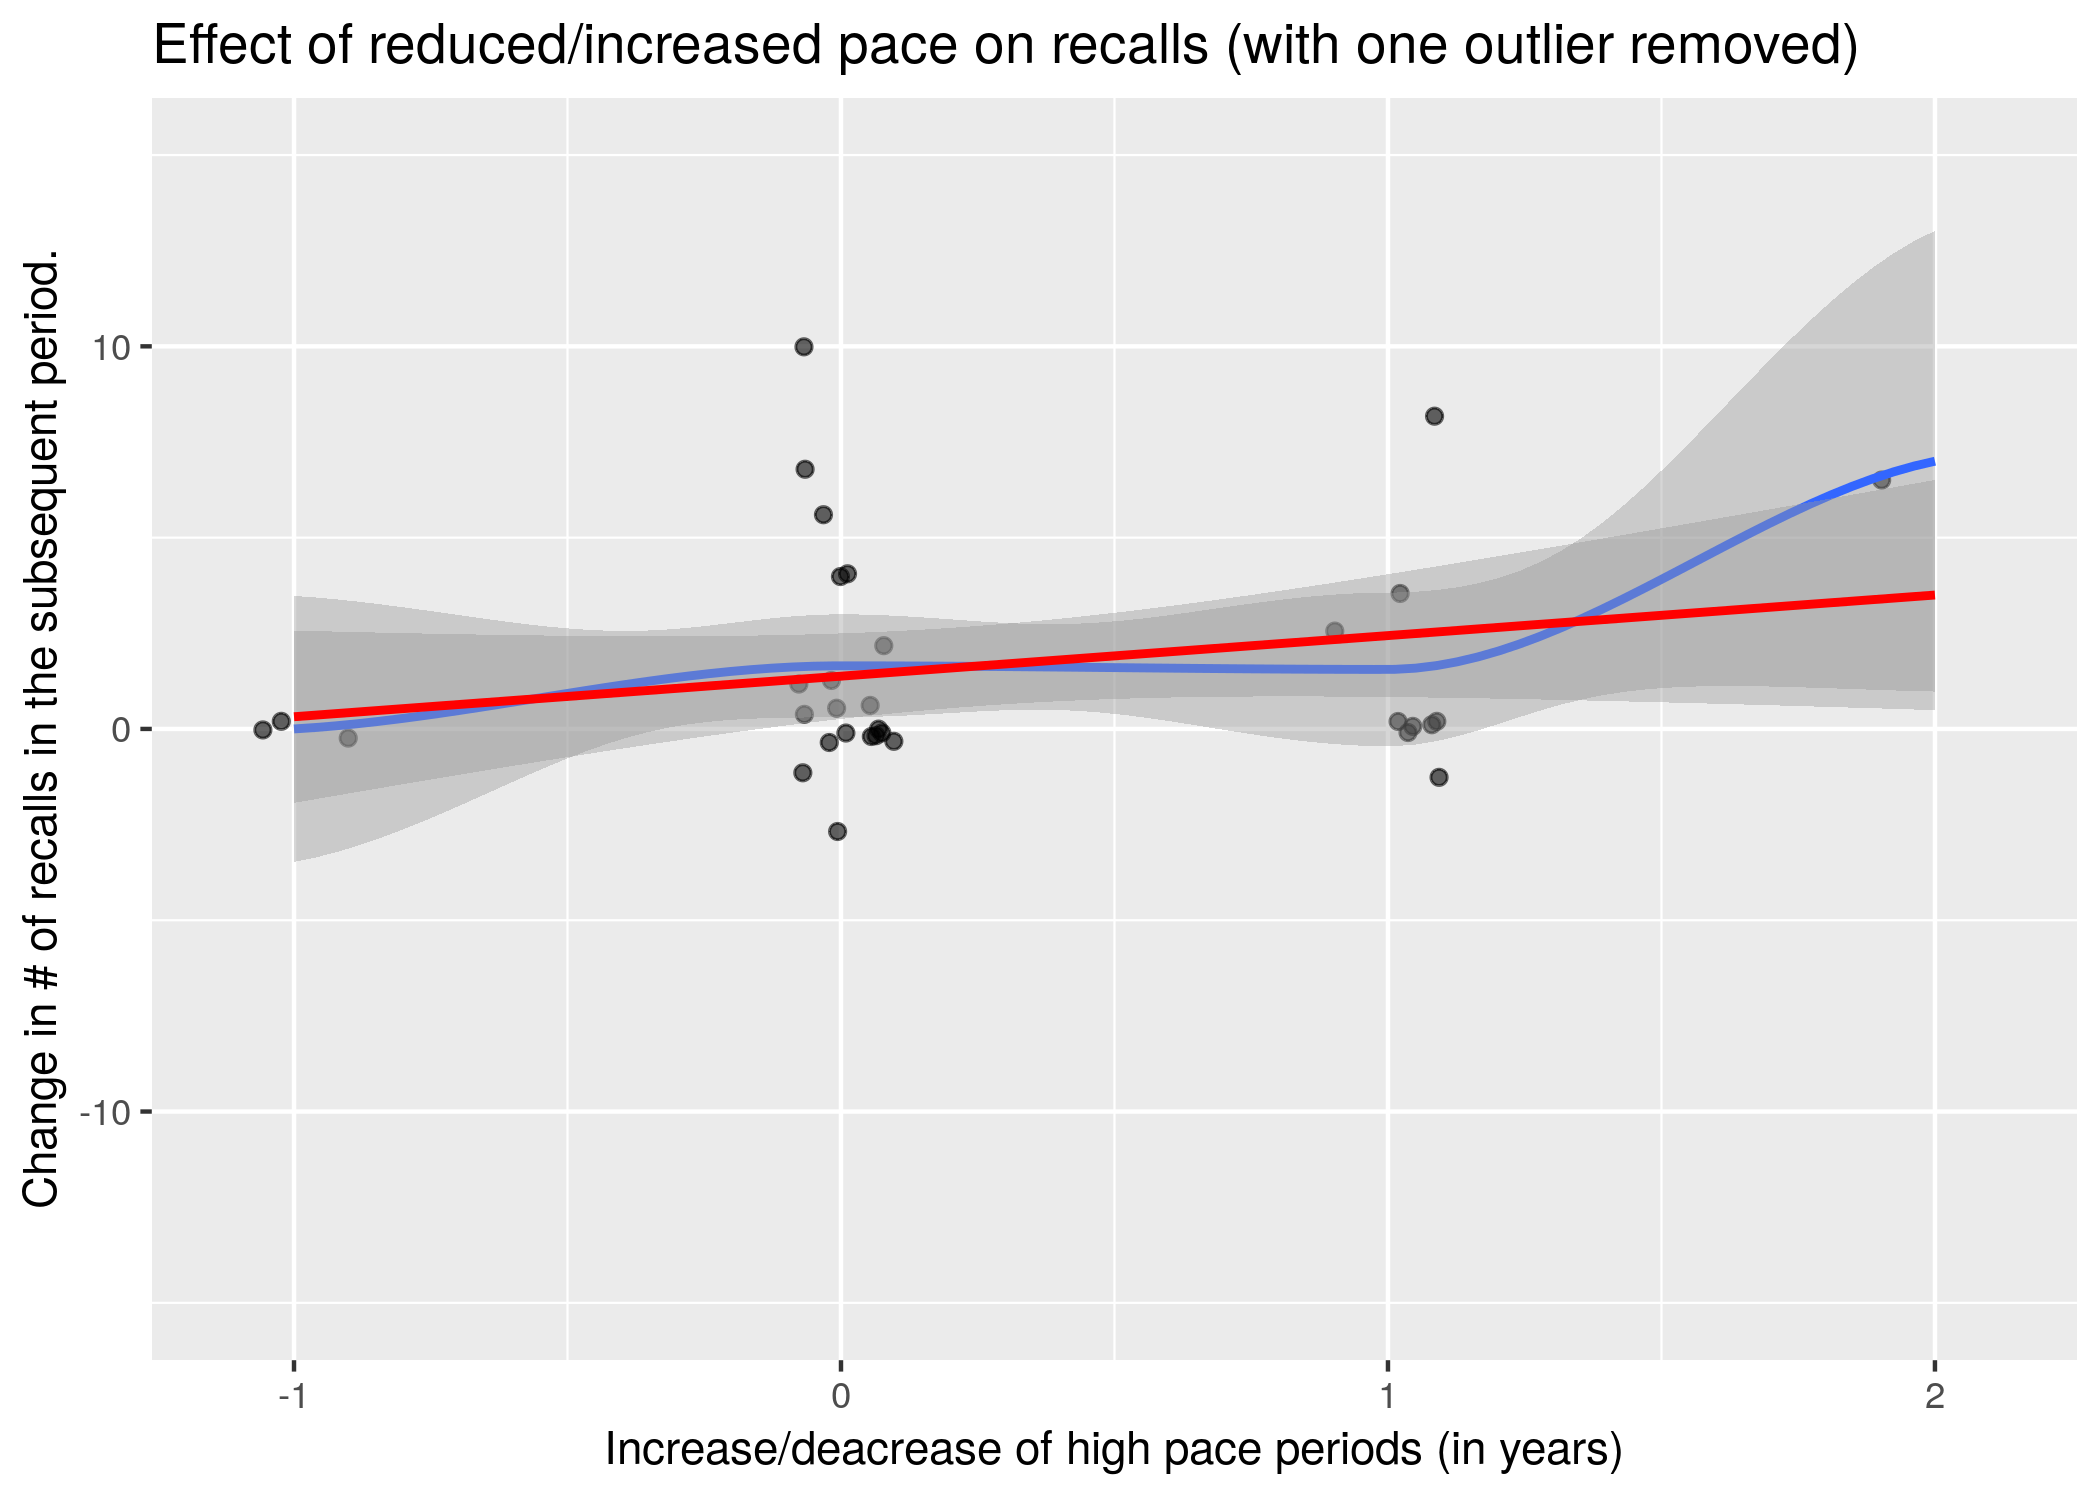
\includegraphics{illustrations/graph2.png}
\end{figure}

\begin{figure}
	\caption{}
	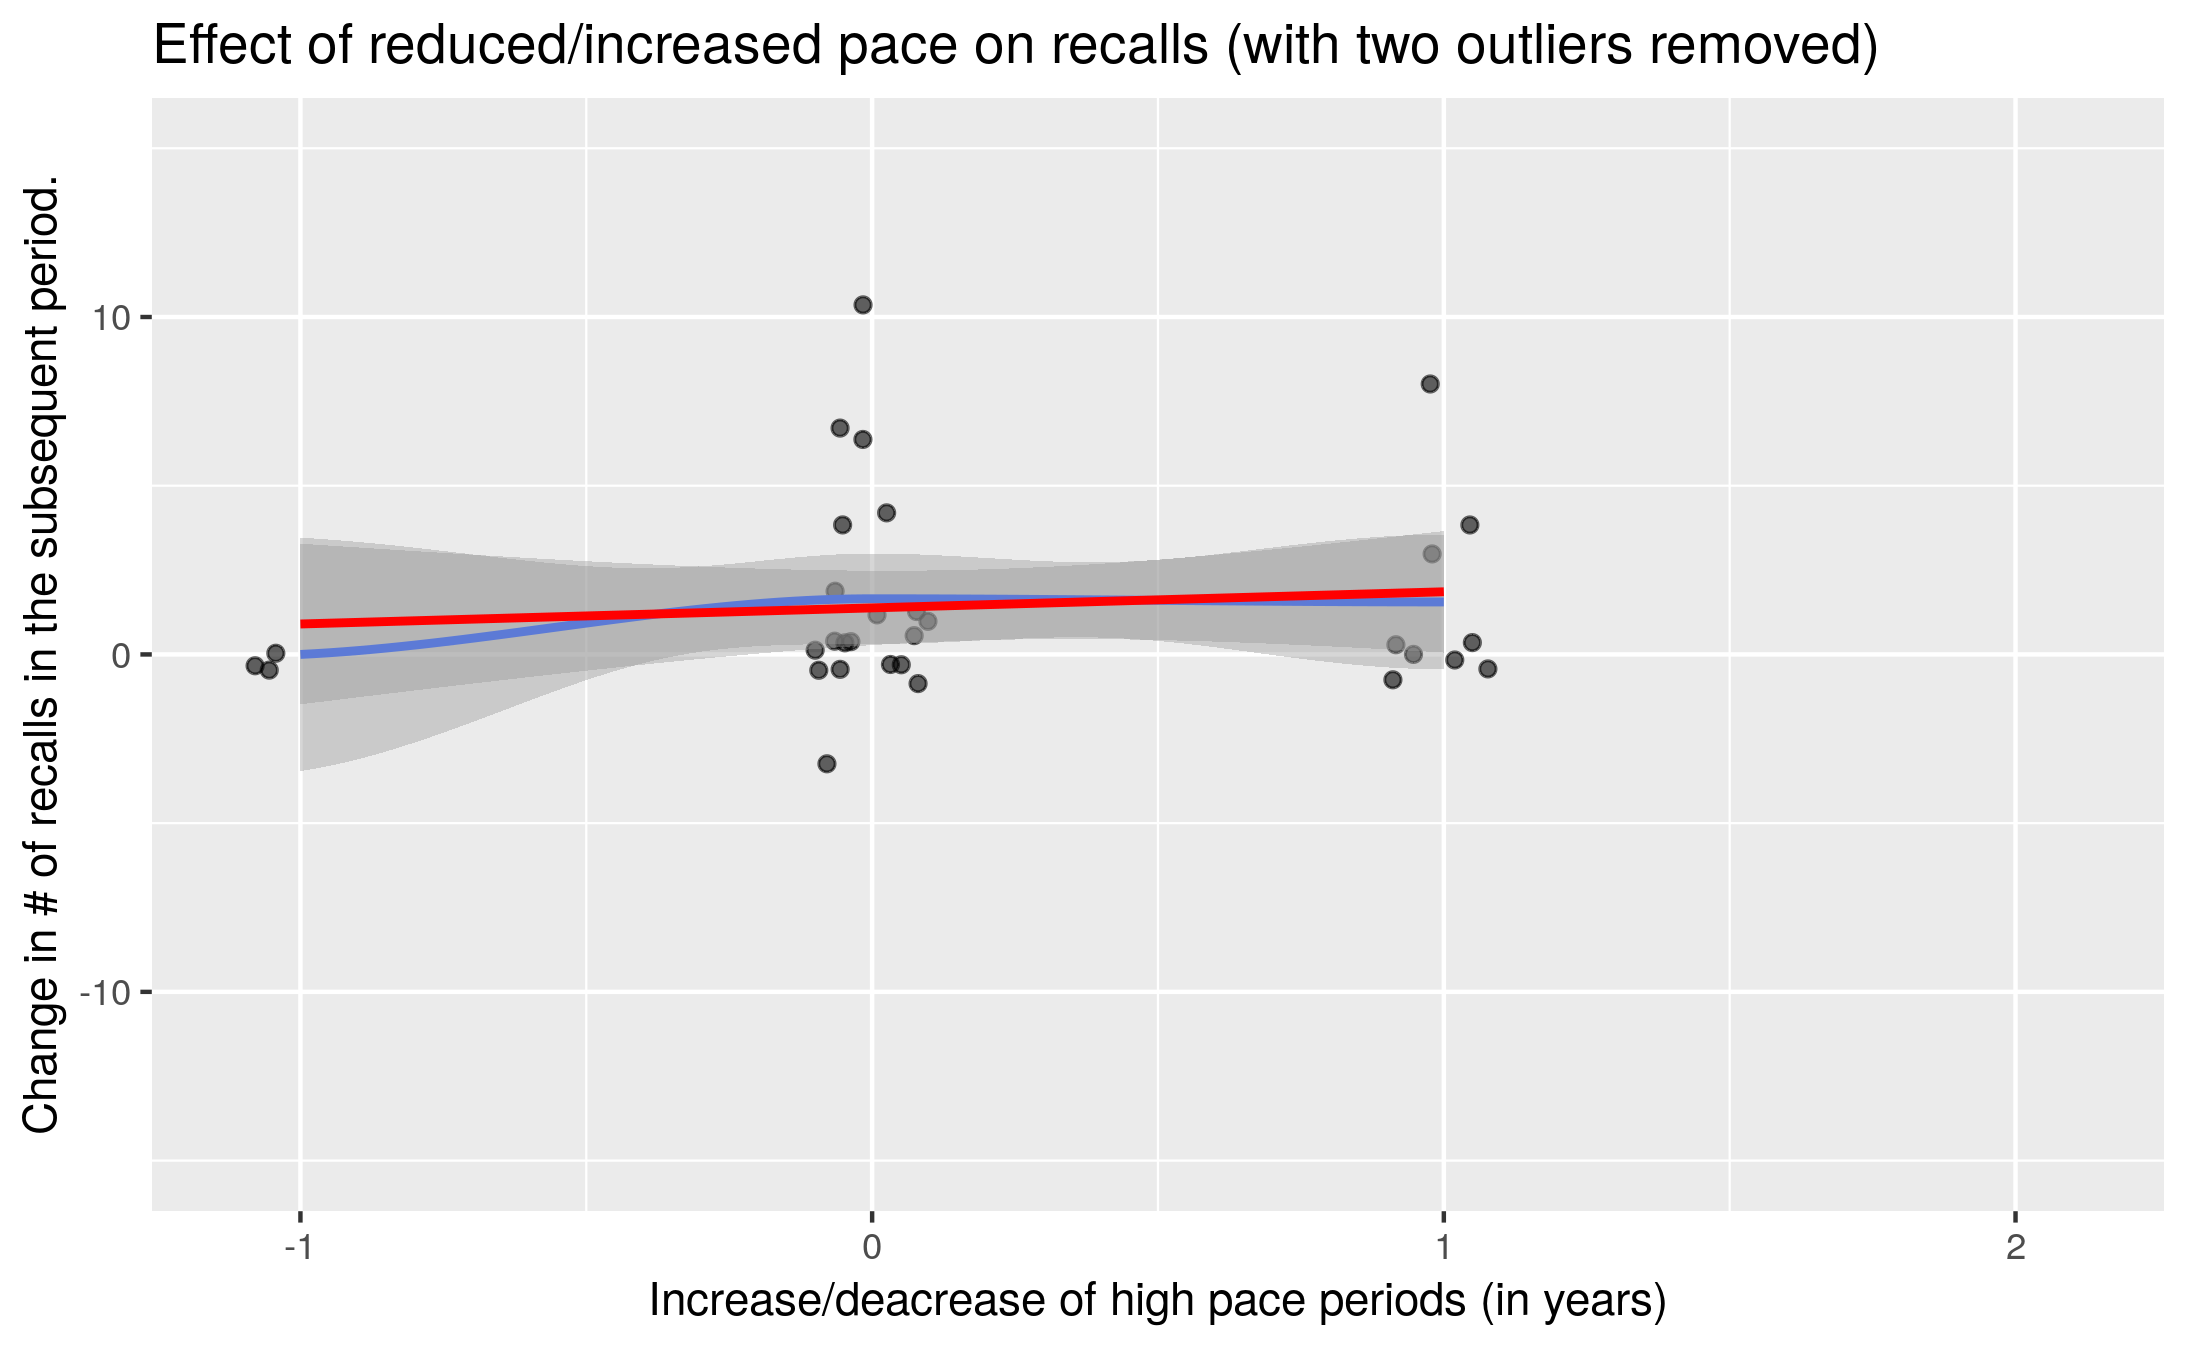
\includegraphics{illustrations/graph3.png}
\end{figure}

